\documentclass[runningheads,a4paper]{llncs}

\usepackage{amssymb}
\setcounter{tocdepth}{3}
\usepackage{graphicx}
\usepackage[spanish]{babel}
\usepackage[utf8]{inputenc}
\usepackage{hyperref}

\usepackage{url}
\newcommand{\keywords}[1]{\par\addvspace\baselineskip
\noindent\keywordname\enspace\ignorespaces#1}
\renewcommand{\keywordname}{\textbf{Palabras clave}:}

\newenvironment{englishabstract}{%
    \renewcommand{\abstractname}{Abstract}% Cambiar el nombre del abstract
    \begin{abstract}%
}{%
    \end{abstract}%
}

\begin{document}

\mainmatter  % start of an individual contribution

% first the title is needed
\title{Hibridación de técnicas de Sistemas de Recomendación. Ventajas del enfoque probabilístico en comparación con la factorización matricial. Implementación del algoritmo Naive Bayes Collaborative Filtering y su expansión para realizar recomendaciones a grupos de usuarios.}

% a short form should be given in case it is too long for the running head
\titlerunning{Hibridación de Técnicas en Sistemas de Recomendación}


\author{Daniel Machado Pérez\\
Osvaldo R. Moreno Prieto\\
Daniel Toledo Martínez}

\authorrunning{\textit{Naive Bayes Collaborative Filtering} expandido con \textit{Naive Pooling}}
% (feature abused for this document to repeat the title also on left hand pages)


\institute{Facultad de Matemática y Computación, Universidad de La Habana, Cuba.\\
\url{https://github.com/DanielMPMatCom/SRI-Project.git}}



\maketitle


\begin{abstract}
  El presente trabajo explora la hibridación de 
  técnicas en sistemas de recomendación, centrándose 
  en las ventajas del enfoque probabilístico frente a 
  la factorización matricial en cuanto a filtrado colaborativo. Se destaca cómo el 
  enfoque probabilístico, al proporcionar una 
  representación explícita de las incertidumbres, 
  mejora la interpretabilidad y explicación de las 
  recomendaciones generadas. En particular, 
  se implementa el algoritmo \textit{Naive Bayes Collaborative Filtering} (NBCF), 
  que combina la simplicidad del modelo \textit{Naive Bayes} 
  con el poder del filtrado colaborativo, 
  permitiendo recomendaciones precisas y explicativas. 
  Además, se expande este algoritmo para adaptarse 
  a la recomendación a grupos de usuarios, 
  abordando un área clave en la personalización 
  colectiva de contenidos. Los resultados demuestran 
  que el enfoque probabilístico no solo ofrece una 
  alternativa robusta a la factorización matricial, 
  sino que también potencia la capacidad del sistema 
  para ofrecer recomendaciones personalizadas y 
  comprensibles, tanto a individuos como a grupos.
\keywords{Sistemas de Recomendación (RS), Filtrado Colaborativo (CF), Enfoque Probabilístico, Factorización Matricial, \textit{Naive Bayes Collaborative Filtering} (NBCF), \textit{Naive Pooling} (NBP).}

\end{abstract}

\begin{englishabstract}
  This work explores the hybridization of techniques 
  in recommendation systems, focusing on the 
  advantages of the probabilistic approach over 
  matrix factorization in collaborative filtering. 
  It highlights how the probabilistic approach, 
  by providing an explicit representation of 
  uncertainties, improves the interpretability and 
  explanation of the generated recommendations. 
  In particular, the Naive Bayes Collaborative 
  Filtering (NBCF) algorithm is implemented, 
  combining the simplicity of the Naive Bayes model 
  with the power of collaborative filtering, 
  allowing for precise and explanatory 
  recommendations. Additionally, this algorithm is 
  expanded to adapt to group recommendations, 
  addressing a key area in the collective 
  personalization of content. The results 
  demonstrate that the probabilistic approach not 
  only offers a robust alternative to matrix 
  factorization but also enhances the system's 
  ability to deliver personalized and understandable 
  recommendations to both individuals and groups.
\end{englishabstract}

\section{Introducción}

En la era de la información, el acceso a grandes volúmenes de datos ha transformado la manera en que los usuarios interactúan con los contenidos en línea. Plataformas como servicios de \textit{streaming}, comercio electrónico, redes sociales y sitios de reseñas, enfrentan el desafío de presentar información relevante de manera eficiente y personalizada. Ante este reto, los sistemas de recomendación han emergido como una herramienta clave para filtrar y personalizar las interacciones de los usuarios, facilitando la identificación de productos, servicios o contenidos acordes a sus preferencias.

A lo largo de los años, diversas técnicas de recomendación han sido desarrolladas y perfeccionadas para abordar este problema, desde enfoques clásicos como el filtrado colaborativo, hasta métodos más sofisticados que combinan varios enfoques en un esquema híbrido. Sin embargo, muchos de estos enfoques, en particular la factorización matricial, presentan limitaciones en términos de explicabilidad, lo que dificulta la interpretación de las recomendaciones ofrecidas.

En este contexto, el presente trabajo se enfoca en la hibridación de técnicas de recomendación, comparando las ventajas del enfoque probabilístico frente a la factorización matricial en sistemas de filtrado colaborativo. El enfoque probabilístico, a través del algoritmo \textit{Naive Bayes Collaborative Filtering} (NBCF) \cite{nbcf}, no solo ofrece una mayor capacidad para manejar incertidumbres en las predicciones, sino que también proporciona explicaciones más comprensibles para los usuarios, mejorando la confianza en las recomendaciones. 

El objetivo de este trabajo es implementar y evaluar un sistema de recomendación que combine técnicas probabilísticas y de filtrado colaborativo, con una extensión particular para abordar las recomendaciones a grupos de usuarios, un área poco explorada pero de creciente relevancia en la personalización colectiva.

Para cumplir con este objetivo, se pretende:
\begin{itemize}
    \item Comparar las ventajas del enfoque probabilístico con la factorización matricial en términos de precisión y explicabilidad.
    \item Implementar el algoritmo NBCF y extenderlo utilizando el enfoque \textit{Naive Pooling} (NBP) \cite{nbp} para realizar recomendaciones efectivas a grupos de usuarios.
    \item Evaluar el rendimiento del sistema propuesto utilizando un conjunto de datos real y métricas estándar de evaluación.
\end{itemize}

La extensión del NBCF para la recomendación grupal 
se basa en el método \textit{Naive Pooling}, 
que combina las probabilidades individuales (que calcularemos 
con NBCF) para generar una recomendación colectiva coherente. Esta extensión permite realizar recomendaciones que reflejan tanto las preferencias individuales como las del grupo, y es particularmente útil en contextos donde se debe personalizar contenido para familias, grupos de amigos o equipos de trabajo.

El presente informe se estructura de la siguiente manera: en el \textbf{Estado del Arte} se revisa la literatura sobre técnicas de recomendación, con un enfoque en el filtrado colaborativo y los modelos probabilísticos. En la sección \textbf{Algoritmo NBCF} se detalla la implementación del algoritmo, mientras que en \textbf{Expansión del Algoritmo NBCF} se describe cómo se adapta este modelo para realizar recomendaciones a grupos de usuarios. Posteriormente, en \textbf{Evaluación de los Resultados}, se presentan y analizan los resultados obtenidos tras la implementación. Finalmente, en las \textbf{Conclusiones}, se resumen los hallazgos más relevantes y se proponen posibles direcciones para investigaciones futuras.

\section{Estado del Arte}

En la era de la información, los sistemas de 
recomendación han surgido como herramientas 
fundamentales para la personalización de contenidos 
y productos, ofreciendo a los usuarios la 
capacidad de descubrir ítems relevantes entre un 
vasto conjunto de opciones. Estos sistemas se han 
implementado en una variedad de sectores, desde 
plataformas de \textit{streaming} de video hasta 
comercios electrónicos, y su evolución ha dado 
lugar a múltiples enfoques técnicos. Dentro de estos, 
destacan el filtrado colaborativo, el filtrado basado 
en contenido, el filtrado demográfico y los enfoques 
híbridos, cada uno con sus propias ventajas y 
limitaciones.

En particular, el filtrado colaborativo ha demostrado 
ser uno de los métodos más efectivos y populares, 
debido a su capacidad para identificar patrones en 
las interacciones previas de los usuarios y ofrecer 
recomendaciones basadas en similitudes. Este enfoque 
se puede implementar mediante técnicas basadas en 
memoria o modelos, siendo estas últimas más escalables 
y precisas. En esta sección se revisan los avances 
clave en los sistemas de recomendación, con énfasis en 
los modelos probabilísticos y sus aplicaciones.

\subsection{Técnicas de Recomendación}

\begin{itemize}
    \item \textbf{Filtrado Colaborativo}: 
    Este enfoque parte de la premisa de que los 
    usuarios con preferencias similares en el pasado 
    coincidirán en sus elecciones futuras. Existen dos 
    variantes principales: el filtrado colaborativo 
    basado en memoria y el basado en modelos. Mientras 
    que el primero utiliza directamente las 
    interacciones previas para hacer recomendaciones, 
    el segundo crea representaciones abstractas que 
    capturan relaciones entre usuarios e ítems, lo que 
    permite una mayor escalabilidad. \cite{estado_arte_sistemas_recomendacion}
    
    \item \textbf{Filtrado Basado en Contenido}: A diferencia del filtrado colaborativo, este método realiza recomendaciones basadas en la similitud entre las características de los ítems que ha consumido previamente un usuario y los ítems disponibles. Esto es común en plataformas que manejan grandes cantidades de datos sobre los atributos de los ítems, como en servicios de streaming de música o video.\cite{estado_arte_sistemas_recomendacion}

    \item \textbf{Filtrado Demográfico}: Aunque menos utilizado, este enfoque se basa en las características personales de los usuarios, como edad, género o ubicación. Si bien puede ser útil en ciertos contextos, su efectividad es limitada al no considerar interacciones directas entre usuarios e ítems.\cite{estado_arte_sistemas_recomendacion}

    \item \textbf{Enfoques Híbridos}: Combinan varios métodos para mejorar la precisión de las recomendaciones. Un ejemplo común es la combinación del filtrado colaborativo con el basado en contenido, lo que permite ofrecer recomendaciones más personalizadas y diversificadas.\cite{estado_arte_sistemas_recomendacion}
\end{itemize}

\subsection{Filtrado Colaborativo Basado en Modelos}

Los métodos basados en modelos han emergido como una solución eficiente para el filtrado colaborativo a gran escala. Dentro de esta categoría, destacan la factorización matricial y los enfoques probabilísticos.

\begin{itemize}
    \item \textbf{Factorización Matricial}: Esta técnica permite descomponer la matriz de interacciones usuario-ítem en matrices de factores latentes, que representan las características no observadas de usuarios e ítems. A pesar de su alta precisión, uno de los desafíos de este enfoque es la falta de interpretabilidad, ya que los factores latentes no siempre son fácilmente comprensibles.\cite{tesis_sistema_recomendador_hibrido}

    \item \textbf{Modelos Probabilísticos}: Una alternativa a la factorización matricial es el uso de modelos probabilísticos, que ofrecen una mayor interpretabilidad al proporcionar explicaciones basadas en probabilidades. Un ejemplo representativo es el \textit{Naive Bayes Collaborative Filtering} (NBCF), que combina la simplicidad del clasificador \textit{Naive Bayes} con el poder del filtrado colaborativo, mostrando resultados prometedores en términos de precisión y eficiencia.\cite{tesis_sistema_recomendador_hibrido}
\end{itemize}

\subsection{Avances en Tesis y Publicaciones Científicas}

El enfoque probabilístico ha sido objeto de un estudio detallado en la tesis doctoral titulada 
``Sistema recomendador híbrido basado en modelos probabilísticos''\cite{tesis_sistema_recomendador_hibrido}. En esta tesis, se aborda la integración de modelos probabilísticos dentro de sistemas de recomendación híbridos, destacando cómo estos modelos no solo permiten una mayor precisión, sino que también aportan una capa de interpretabilidad que los métodos de factorización matricial no ofrecen. El autor propone un enfoque híbrido que combina los beneficios del filtrado colaborativo basado en modelos probabilísticos con técnicas de filtrado basado en contenido.

En el paper titulado ``\textit{Naïve 
Bayes} Extendido para Clasificación Basada en Grupos''\cite{nbp}, los autores presentan una extensión del clásico modelo \textit{Naive Bayes}, adaptándolo para su aplicación en la clasificación basada en grupos. Uno de los enfoques tratados, denominado \textit{Naive Pooling} (NBP), se centra en la agregación de probabilidades individuales para generar una probabilidad conjunta que permita la clasificación efectiva de grupos de usuarios. La metodología propuesta combina las probabilidades individuales de cada miembro del grupo para maximizar la coherencia y relevancia de la clasificación final. Este método resulta particularmente útil en contextos donde se deben generar recomendaciones o decisiones que reflejen tanto las preferencias individuales como la dinámica grupal. La capacidad de NBP para mantener la simplicidad del modelo Naive Bayes, al tiempo que amplía su aplicabilidad a escenarios grupales, lo convierte en una herramienta poderosa para la personalización colectiva en sistemas de recomendación.

Además, en el paper ``Un Enfoque de Filtrado Colaborativo
Basado en un Clasificador \textit{Naive Bayes}''\cite{nbcf}, 
se profundiza en la implementación del NBCF y se demuestra su viabilidad como alternativa a los métodos tradicionales de filtrado colaborativo. Los resultados obtenidos en este estudio muestran que el NBCF puede igualar o superar el rendimiento de la factorización matricial, especialmente en datasets donde la interpretabilidad es tan importante como la precisión.

Finalmente, el trabajo ``Filtrado Colaborativo Híbrido Basado en Interacciones de Usuarios con el Sistema de Votaciones''\cite{hybrid_collaborative_filtering} presenta un enfoque híbrido que integra el comportamiento de valoración de los usuarios con el filtrado colaborativo. Este enfoque tiene una relevancia particular para 
nuestro proyecto, ya que permite ajustar las recomendaciones no solo en función de las interacciones pasadas, sino también considerando la manera en que los usuarios valoran los ítems, lo que aporta una capa adicional de personalización.

\subsection{Trabajos Recientes y Aplicaciones Actuales}

En la actualidad, los sistemas de recomendación han 
expandido su campo de aplicación y han adoptado nuevas 
tecnologías para mejorar su rendimiento. Una de las 
áreas emergentes es el uso de \textit{hardware} reconfigurable 
para acelerar los cálculos necesarios en estos 
sistemas. Según Pajuelo Holguera \cite{TDUEX_2021_Pajuelo_Holguera}, 
el uso de FPGAs ha mostrado ser una solución eficiente 
para reducir los tiempos de procesamiento en sistemas 
de recomendación, especialmente en escenarios de 
grandes volúmenes de datos. Su trabajo también explora 
cómo los sistemas de recomendación pueden ser 
aplicados en entornos sensoriales para predecir 
variables ambientales, abriendo nuevas oportunidades 
en el ámbito de las ciudades inteligentes.

Por otro lado, el trabajo de César 
Pita \cite{_Cesar_Enrique_Pita_Perez} resalta cómo 
la combinación de técnicas de \textit{Machine Learning} 
con sistemas de recomendación híbridos mejora 
significativamente la predicción de preferencias de 
usuarios. Al integrar características demográficas, 
históricas y basadas en contenido, estos modelos 
ofrecen recomendaciones más ajustadas incluso en 
escenarios con datos limitados.

Estos trabajos representan un avance importante 
en la mejora de la eficiencia y precisión de los 
sistemas de recomendación, abriendo el camino a 
nuevas aplicaciones en campos como el control 
ambiental, la interacción sensorial y la 
personalización grupal en plataformas de alto 
volumen de datos.


\section{Algoritmo NBCF}

El algoritmo NBCF constituye una estrategia eficiente 
y novedosa dentro del ámbito de los sistemas de 
recomendación colaborativos. A continuación, se 
presenta una revisión detallada de los fundamentos 
teóricos y matemáticos que sustentan este enfoque, 
así como una descripción de su implementación práctica 
y los resultados obtenidos en diferentes estudios 
experimentales.

\subsection{Introducción al Algoritmo NBCF}

El algoritmo \textit{Naive Bayes Collaborative 
Filtering} (NBCF) es una técnica innovadora dentro 
del campo de los sistemas de recomendación 
colaborativos. A diferencia de otros enfoques, 
como la factorización matricial, el NBCF aprovecha la 
simplicidad y efectividad del clasificador \textit{Naive Bayes} 
para predecir las preferencias de los usuarios en 
función de sus interacciones anteriores con ítems. 
Este método considera la probabilidad de que un 
usuario asigne una cierta calificación a un ítem, 
basándose en las calificaciones previas tanto del 
usuario como de otros usuarios con comportamientos 
similares.

\subsection{Formulación Matemática del Algoritmo NBCF}

El algoritmo NBCF se basa en la combinación de dos 
enfoques principales: basado en usuarios y basado 
en ítems. En cada uno de estos enfoques, se calcula la 
probabilidad a priori de que un usuario califique un 
ítem con un valor específico, y posteriormente se 
calcula el \textit{likelihood} para ajustar esta 
probabilidad en función de las calificaciones 
observadas.

\begin{itemize}
    \item \textbf{Enfoque basado en el usuario}:
    la probabilidad a priori y el \textit{likelihood} se
    calculan de acuerdo con los ítems que cada usuario ha votado. \cite{tesis_sistema_recomendador_hibrido}
    \item \textbf{Enfoque basado en ítems}:
    la probabilidad a priori y el \textit{likelihood} se calculan
    de acuerdo con los votos que cada ítem ha recibido. \cite{tesis_sistema_recomendador_hibrido}
    \item \textbf{Enfoque híbrido}:
    integra los enfoques basados en el usuario e ítems, a fin
    de complementarse uno con otro y mejorar la precisión del modelo. \cite{tesis_sistema_recomendador_hibrido}

\end{itemize}

Para el desarrollo de cada uno de estos enfoques se 
utiliza los siguientes conceptos de probabilidades:

\begin{itemize}
    \item \textbf{Probabilidad A Priori}: 
    En el enfoque basado en ítems, se calcula la 
    probabilidad a priori de que un usuario $u$ asigne 
    una calificación $y$ a un ítem $i$, 
    denotado como $P(r_u = y)$. De manera análoga, 
    en el enfoque basado en usuarios, se calcula la 
    probabilidad de que un ítem $i$ reciba una 
    calificación $y$ de cualquier usuario $u$, 
    denotado como $P (r_i = y)$.\\

    \begin{equation}
        P(r_i = y) = \frac{|\{u \in U|r_{u,i} = y\}| + \alpha}{|\{u \in U|r_{u,i} \neq \bullet\}| + |R|*\alpha}
    \end{equation} \cite{tesis_sistema_recomendador_hibrido}

    Donde:
    \begin{itemize}
        \item $U$ es el conjunto de usuarios.
        \item $r_{u,i}$ es la calificación otorgada por el usuario $u$ al ítem $i$.
        \item $\alpha$ es un parámetro para evitar 0 probabilidades.
        \item $|R|$ representa el número de votos plausibles.
        \item $\bullet$ representa la ausencia de voto.
    \end{itemize} 

    
    \item \textbf{Likelihood}: 
    El \textit{likelihood} ajusta la probabilidad a 
    priori mediante la consideración de la 
    información adicional disponible en las 
    calificaciones observadas. Para el enfoque basado 
    en ítems, esto se expresa como 
    $P(r_v = k | r_u = y)$, que representa la 
    probabilidad de que otro usuario $v$ califique 
    con $k$ un ítem que ha sido calificado con $y$ 
    por el usuario $u$. Similarmente, para el enfoque 
    basado en usuarios, se calcula el \textit{likelihood} 
    correspondiente $P(r_j = k|r_i = y)$.

    \begin{equation}
        P(r_j = k|r_i = y) =  \\ \frac{|\{u \in U|r_{u,j} = k  \land  r_{u,i} = y\}|+ \alpha}{|\{u \in U|r_{u,j} \neq \bullet \land r_{u,i} = y|\} + |R|*\alpha}
    \end{equation} \cite{tesis_sistema_recomendador_hibrido}


    
    \item \textbf{Combinación de Enfoques}: 
    En el enfoque híbrido, se integran las 
    probabilidades obtenidas de los enfoques basados 
    en usuarios y en ítems, proporcionando un modelo 
    más robusto y preciso para la predicción de 
    calificaciones.

    $P(r_{u,i} = y)$ representa el valor de
    probabilidad de que el usuario $u$ vote el ítem $i$ 
    con el voto $y$:
\begin{small}
    \begin{equation}
        P(r_{u,i} = y) \propto \\ \left( P(r_u = y) \cdot \prod_{v \in Ui} P(r_v = r_{v,i} | r_u = y) \right)^{\frac{1}{1+|Ui|}} \\
        \cdot \left( P(r_i = y) \cdot \prod_{j \in Iu} P(r_j = r_{u,j} | r_i = y) \right)^{\frac{1}{1+|Iu|}}
    \end{equation} \cite{tesis_sistema_recomendador_hibrido}
    
\end{small}

    Donde:
    \begin{itemize}
        \item $I_u = \{i \in I \mid r_{u,i} \neq \bullet \}$ es el conjunto de ítems votados por el usuario $u$,
        \item y $U_i = \{u \in U \mid r_{u,i} \neq \bullet \}$ es el conjunto de usuarios que han votado el ítem $i$.
    \end{itemize} 
\end{itemize}
 

\subsection{Algoritmo NBCF: Implementación Paso a Paso}

El algoritmo NBCF se implementa de manera iterativa, 
asegurando la eficiencia computacional mediante 
técnicas de memorización que permiten evitar el 
recálculo innecesario de probabilidades. 
A continuación se describen los pasos del algoritmo:

\begin{itemize}
    \item \textbf{Inicialización}: 
    Se inicializan las probabilidades a priori y los 
    contadores utilizados en el cálculo de 
    \textit{likelihoods}.
    \item \textbf{Iteración sobre Usuarios e Ítems}: 
    Para cada usuario, se calcula la probabilidad de 
    cada calificación posible basada en las 
    calificaciones observadas para los ítems que 
    ha evaluado. De manera similar, se calcula para 
    cada ítem la probabilidad de recibir una 
    calificación específica basada en las 
    calificaciones anteriores recibidas.
    \item \textbf{Almacenamiento de Resultados}: 
    Los valores calculados se almacenan para ser 
    utilizados posteriormente en la predicción de 
    nuevas calificaciones, evitando la necesidad de 
    recalcular durante la fase de predicción.
\end{itemize}

Este enfoque garantiza que el NBCF no solo sea 
eficiente, sino que también se adapte bien a problemas 
de gran escala, manteniendo una complejidad 
computacional similar a la de otros métodos avanzados, 
como la factorización matricial \cite{tesis_sistema_recomendador_hibrido}.

\subsection{Resultados Experimentales y Comparativa}

El algoritmo NBCF ha demostrado su eficacia en 
múltiples conjuntos de datos públicos 
(MovieLens, FilmTrust, Yahoo, BookCrossing)\cite{tesis_sistema_recomendador_hibrido}, superando en 
varias métricas clave a los métodos de referencia más 
utilizados en el campo:
\begin{itemize}
    \item Error Medio Absoluto (MAE) \cite{tesis_sistema_recomendador_hibrido}
    \item Precisión y \textit{Recall} \cite{tesis_sistema_recomendador_hibrido}
    \item Ganancia acumulada descontada normalizada (nDCG) \cite{tesis_sistema_recomendador_hibrido}
\end{itemize}
Se compararon los siguientes enfoques:
\begin{itemize}
    \item NBCF (usuario)
    \item NBCF (ítem)
    \item NBCF (híbrido)
    \item BNMF
    \item GGM
    \item INBM
    \item Bi-CF
    \item NMF
\end{itemize}
Los resultados fueron los siguientes:
\begin{itemize}
    \item \textbf{MovieLens}: El enfoque 
    híbrido de NBCF ha mostrado mejoras significativas en 
    medidas de MAE, precisión y \textit{recall}, 
    así como el enfoque basado en ítems fue mejor en la 
    nDCG en comparación con enfoques 
    tradicionales.\cite{tesis_sistema_recomendador_hibrido}
    \item \textbf{FilTrust}: el MAE de NBCF (híbrido) 
    logra mejores resultados que los otros dos enfoques 
    propuestos, mientras que la precisión y recall son 
    mejores con NBCF (ítems) y NBCF (usuario). 
    Por otro lado, cuando aumenta el número de 
    recomendaciones, nDCG es mejor con el enfoque NBCF (híbrido).\cite{tesis_sistema_recomendador_hibrido}
    \item \textbf{Yahoo}: nDCG es mejor en NBCF
    (híbrido) en comparación con NBCF (ítem) y NBCF (usuario). 
    Además, la precisión y el \textit{recall} de los 
    tres enfoques propuestos presentan un resultado 
    casi similar entre ellos. Así mismo, hay una 
    superioridad lograda en MAE de NBCF (híbrido)
    con respecto a los otros enfoques propuestos.\cite{tesis_sistema_recomendador_hibrido}
    \item \textbf{BookCrossing}: NBCF (híbrido) y NBCF (ítem)
    proveen mejores resultados para nDCG en 
    comparación con los métodos de línea base de CF. 
    A diferencia de otros conjuntos de datos en 
    BookCrossing las métricas de precisión y \textit{recall} 
    son mejores para los métodos GGM, INBM y Bi-CF. 
    Sin embargo muestran una mejora con respecto a 
    los métodos BNMF y NMF. NBCF (híbrido) se muestra 
    superior al resto de los enfoques en cuanto al MAE.\cite{tesis_sistema_recomendador_hibrido}
\end{itemize}

\subsection{Conclusión}

El algoritmo NBCF representa una mejora significativa 
en el ámbito de los sistemas de recomendación 
colaborativos, combinando la simplicidad del 
clasificador \textit{Naive Bayes} con técnicas de filtrado 
colaborativo para ofrecer recomendaciones precisas y 
eficaces. Su capacidad para integrar múltiples 
enfoques y adaptarse a diferentes escenarios lo 
convierte en una herramienta valiosa para la mejora de 
la experiencia del usuario en plataformas de 
recomendación.

\section{Expansión del Algoritmo NBCF}


El algoritmo NBP, como extensión del enfoque clásico 
\textit{Naive Bayes}, permite abordar la recomendación 
grupal, un desafío creciente en los sistemas de 
recomendación. A continuación, se describe la 
formulación matemática del algoritmo y su integración 
con el modelo NBCF, junto con una discusión de las 
ventajas, limitaciones y detalles de implementación 
que hacen posible la recomendación precisa tanto para 
usuarios individuales como para grupos.

\subsection{Algoritmo NBP. Formulación Matemática}
En los sistemas de recomendación modernos, la 
capacidad de realizar recomendaciones efectivas 
no solo a usuarios individuales, sino también a grupos, 
se ha vuelto un aspecto crucial. Contextos como la 
recomendación de contenido para familias, equipos de 
trabajo o grupos de amigos demandan un enfoque que 
pueda considerar y equilibrar las preferencias 
individuales dentro de un colectivo, maximizando la 
satisfacción general del grupo. En respuesta a esta 
necesidad, surge el algoritmo NBP, una extensión del 
modelo clásico de \textit{Naive Bayes} adaptado 
específicamente para la clasificación y recomendación 
a grupos de usuarios.

El algoritmo se fundamenta en la misma premisa básica 
que el \textit{Naive Bayes}, es decir, la independencia 
condicional de las características dadas las clases. 
Sin embargo, lo que distingue a NBP es su capacidad 
para combinar las probabilidades individuales de los 
miembros de un grupo, produciendo una probabilidad 
conjunta que guía la recomendación o clasificación 
final para todo el grupo.

Matemáticamente, la probabilidad conjunta para un 
grupo $G$ de $n$ usuarios con respecto a una clase $C_l$ 
se puede expresar como:

\begin{equation}
    P(C_l) = \frac{\prod_{k=1}^{n} P(C_l|x_k)}{\prod_{k=1}^{n} P(c_l|x_k) + \prod_{k=1}^{n} (1-P(c_l|x_k))}
\end{equation} \cite{nbp}

Donde:
\begin{itemize}
    \item $x_k$ es un usuario del grupo $G$,
    \item $P(C_l|x_k)$ es la probabilidad de la 
    clase $C_l$ dada para el usuario individual $x_k$. 
\end{itemize} 

El algoritmo NBP maximiza esta probabilidad conjunta, 
seleccionando la clase $C_l$ que mayor valor obtenga, 
lo que se traduce en una recomendación para el grupo 
que refleje un consenso entre las preferencias 
individuales.

\subsection{Ventajas y Desventajas de NBP}

El algoritmo Naive Pooling presenta varias ventajas notables:
\begin{itemize}
    \item \textbf{Simplicidad y Eficiencia}: 
    Al estar basado en el modelo \textit{Naive Bayes}, 
    NBP hereda la simplicidad computacional y la 
    eficiencia del mismo, lo que permite su 
    implementación en sistemas a gran escala sin 
    requerir un costo computacional elevado.
    \item \textbf{Interpretabilidad}:
    Una de las fortalezas del enfoque probabilístico 
    es su capacidad para proporcionar una explicación 
    clara de las recomendaciones basadas en 
    probabilidades. Esto facilita la interpretación de 
    por qué un grupo recibió una recomendación 
    específica.
    \item \textbf{Adaptabilidad}:
    NBP es altamente adaptable y puede integrarse con 
    facilidad en sistemas de recomendación existentes 
    que ya utilicen el enfoque \textit{Naive Bayes} 
    para recomendaciones individuales. Esto permite a 
    los desarrolladores extender sus sistemas a la 
    recomendación grupal sin necesidad de una 
    reingeniería significativa.
\end{itemize}

A pesar de sus ventajas, el algoritmo NBP también 
presenta algunas limitaciones que deben ser consideradas:

\begin{itemize}
    \item \textbf{Suposición de Independencia}:
    Al igual que \textit{Naive Bayes}, NBP asume que 
    las preferencias de los usuarios dentro del grupo 
    son condicionalmente independientes, lo cual puede 
    no reflejar adecuadamente la realidad, donde las 
    preferencias de los usuarios pueden estar 
    correlacionadas.
    \item \textbf{Equidad en la Recomendación}:
    NBP no tiene en cuenta explícitamente la equidad 
    entre las preferencias individuales dentro del 
    grupo. Es decir, podría favorecer las preferencias 
    de algunos usuarios sobre otros, especialmente si 
    las probabilidades individuales de ciertos miembros 
    del grupo son mucho más altas que las de los demás.
    \item \textbf{Escalabilidad con Grupos Grandes}:
    Aunque eficiente, a medida que el tamaño del grupo 
    aumenta, la combinación de probabilidades puede 
    llevar a situaciones donde las recomendaciones 
    sean dominadas por usuarios con preferencias 
    extremas, lo que podría reducir la diversidad y la 
    satisfacción global del grupo.
\end{itemize}

\subsection{Aplicación del Algoritmo NBP en la Expansión de NBCF}

En el contexto de esta investigación, el algoritmo 
\textit{Naive Pooling} se integrará con el modelo 
\textit{Naive Bayes Collaborative Filtering} (NBCF). 
Teniendo previamente calculados los valores de las 
probabilidades para cada usuario con NBCF, ya sea con 
su enfoque basado en usuario, basado en ítems o híbrido,
se puede efectuar la fórmula de NBP y obtener el resultado 
que se quiere. De esta forma, se extiende 
la funcionalidad del NBCF para proporcionar 
recomendaciones no solo a individuos, sino también a 
grupos de usuarios, conservando la precisión y 
explicabilidad del enfoque probabilístico. 
Esta expansión permitirá que el sistema no solo 
mantenga la calidad en las recomendaciones 
individuales, sino que también pueda satisfacer las 
necesidades de colectivos en situaciones donde la 
personalización grupal es esencial.

\subsection{Detalles de Implementación}

Para la evaluación de la implementación y expansión 
del algoritmo NBCF, se ha seleccionado el dataset 
FilmTrust\cite{filmtrust}, un conjunto de datos ampliamente utilizado 
en la investigación de sistemas de recomendación. 
FilmTrust contiene miles de calificaciones de 
películas proporcionadas por usuarios, lo que lo 
convierte en un recurso valioso para el análisis y 
desarrollo de modelos de recomendación. 
La riqueza y diversidad del dataset permiten probar 
la eficacia de los algoritmos en un entorno 
cercano a escenarios del mundo real. 
Este dataset fue uno de los utilizados en la tesis antes mencionada.


\section{Evaluación de los resultados}

En esta sección se presentará la evaluación del 
rendimiento de la expansión del algoritmo NBCF para 
la recomendación a grupos utilizando el algoritmo NBP. 
Para ello, se ha seleccionado el dataset \textit{FilmTrust}
 por sus características particulares y su amplio uso 
 en investigaciones de sistemas de recomendación.

 \subsection{Descripción del dataset \textit{FilmTrust}}

 El dataset \textit{FilmTrust} contiene información 
 sobre la interacción de usuarios con películas, 
 lo cual lo convierte en un recurso valioso para el 
 análisis de sistemas de recomendación. 
 Sus características principales son las siguientes:
 \begin{itemize}
    \item \textbf{1508 usuarios}: Cada usuario ha 
    evaluado uno o varios ítems (películas) del conjunto.
    \item \textbf{2071 ítems}: El conjunto de ítems representa las películas que los usuarios han visto y valorado.
    \item \textbf{35494 votos}: Los usuarios han emitido un total de 35,494 calificaciones sobre las películas del conjunto.
    \item \textbf{Escala de votación}: Las calificaciones originales varían entre 0.5 y 4, con incrementos de 0.5. Para simplificar la indexación y el procesamiento en la implementación del sistema, se ha multiplicado la escala por 2, de modo que las calificaciones oscilan entre 1 y 8, con incrementos de 1. Esto permite una mayor precisión y facilidad a la hora de manejar los datos.
    \item \textbf{Dispersión del dataset}: El valor de dispersión (\textit{sparsity}) de este conjunto es del 98.86\%. Esto significa que la mayoría de las posibles combinaciones entre usuarios e ítems no tienen una calificación registrada, lo que introduce un desafío significativo para el modelo de recomendación. La sparsity es una medida que refleja el nivel de dispersión de los datos en una matriz de interacciones usuario-ítem, donde un valor elevado indica que muchas de las posiciones en la matriz están vacías, es decir, no contienen interacciones registradas. Este fenómeno es común en sistemas de recomendación, y requiere el uso de modelos capaces de manejar eficazmente la falta de datos.
 \end{itemize}

 \subsection{Diseño del test}
 Dado que no se encontró un dataset disponible que incluyera información sobre recomendaciones realizadas a grupos de usuarios, surgió la necesidad de diseñar un test propio que permitiera evaluar la efectividad del método propuesto para recomendaciones grupales. El enfoque adoptado utiliza el conjunto de datos de \textit{FilmTrust}, donde se ha adaptado la estructura del dataset para generar grupos de usuarios con características comunes.

 \subsubsection{Confección de los grupos de usuarios}
 A partir de cada película en el dataset, se forma un grupo compuesto por todos los usuarios que le han asignado la misma calificación. Este proceso garantiza que los grupos compartan una opinión similar sobre el ítem en cuestión, lo que es relevante para medir la coherencia del sistema de recomendación en entornos colaborativos. Una vez conformados los grupos iniciales, de cada uno se selecciona aleatoriamente un subconjunto de usuarios, que constituirá uno de los grupos finales sobre los que se realizarán las evaluaciones.

En particular, se pone énfasis en la evaluación de la eficacia del método para grupos que hayan otorgado altas calificaciones a las películas (valores de 6, 7 u 8 en la escala de votos) y bajas calificaciones (1, 2, 3). Esto permite analizar el rendimiento del algoritmo en escenarios donde existe un fuerte consenso positivo entre los usuarios, lo que representa un caso de uso frecuente en las recomendaciones de contenido audiovisual para grupos de amigos o familiares.
Es válido señalar que de esta forma de armar los grupos, pueden existir intersecciones entre ellos, lo cual se ajusta a los escenarios reales y no provoca dificultades para el desempeño del método propuesto. La semilla para replicar los experimentos fue 42.
 
\subsubsection{Procedimiento}

Una vez conformados los grupos de usuarios que han calificado de manera idéntica una película en particular, se procede a eliminar la información de los votos emitidos por esos usuarios hacia dicha película. Este paso es fundamental para simular un escenario en el que los miembros del grupo no han visto la película, lo cual nos permite evaluar la capacidad del sistema de realizar recomendaciones grupales efectivas.

Es importante destacar que la razón de la selección de subconjuntos de usuarios de los grupos iniciales es evitar la pérdida completa de la información relacionada con los votos de la película. De esta manera, se conserva parte de la información del ítem en cuestión, lo que nos permite continuar utilizando el resto de las interacciones de los usuarios con otras películas en el proceso de recomendación.

El objetivo de este procedimiento es evaluar si, bajo la suposición de que los usuarios del grupo no han visto la película, el sistema es capaz de predecir una calificación grupal similar a la calificación inicial. Dado que los miembros del grupo han otorgado una calificación uniforme a la película antes de eliminar esta información, se espera que el sistema de recomendación prediga un voto grupal consistente con las valoraciones originales. Además, al aplicar este procedimiento a películas que recibieron calificaciones altas (6, 7 u 8), se puede evaluar la capacidad del modelo para recomendar este tipo de películas en escenarios donde los usuarios no las hayan visto. De la misma forma al comprobar el rendimiento con las bajas calificaciones (1, 2, 3) se analiza su efectividad para no recomendar películas que no serían bien calificadas por los integrantes del grupo.

\subsubsection{Resultados con votaciones altas (6, 7, 8)\\}

\textbf{Diferencias}

En la Figura \ref{fig:diferencias}, se muestran las diferencias entre las recomendaciones sugeridas por el sistema y las expectativas del usuario. Este gráfico permite identificar las desviaciones del sistema con respecto a las preferencias reales, lo que ofrece una visión clara de las áreas donde se puede mejorar la precisión de las recomendaciones.

\begin{figure}[h]
    \centering
    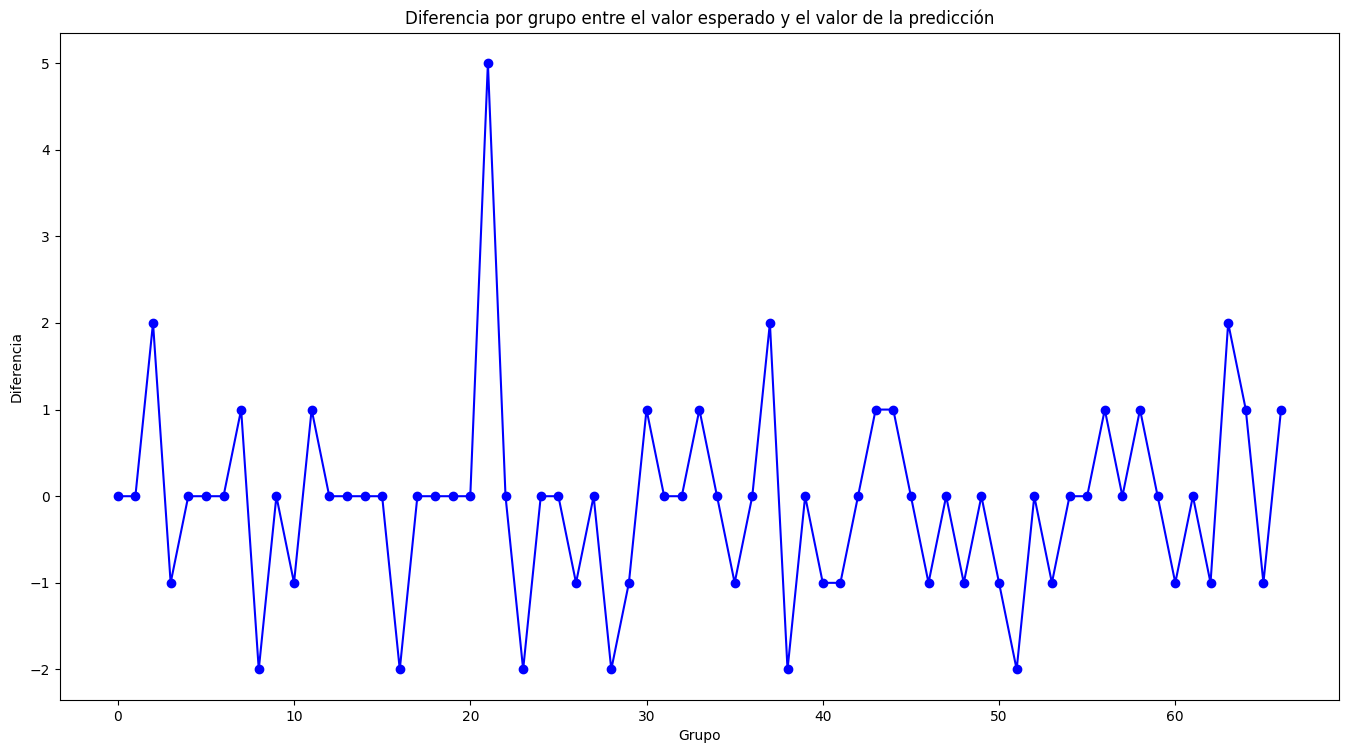
\includegraphics[width=\columnwidth]{assets/Diferencias678.png}
    \caption{Gráfico de diferencias entre las recomendaciones del sistema y las preferencias reales del usuario. Calificaciones 6, 7, 8.}
    \label{fig:diferencias}
\end{figure}

El análisis de estas diferencias sugiere que, si bien el sistema tiende a alinearse con las preferencias de los usuarios en un número considerable de casos, persisten desviaciones en ciertos grupos.

\textbf{Diferencias absolutas}

La Figura \ref{fig:absolutas} muestra las diferencias absolutas, es decir, el valor absoluto de la desviación entre las recomendaciones sugeridas y las expectativas del usuario. Esta representación visual permite observar cuán grandes son las desviaciones sin tener en cuenta la dirección (positiva o negativa) de la diferencia.

\begin{figure}[h]
    \centering
    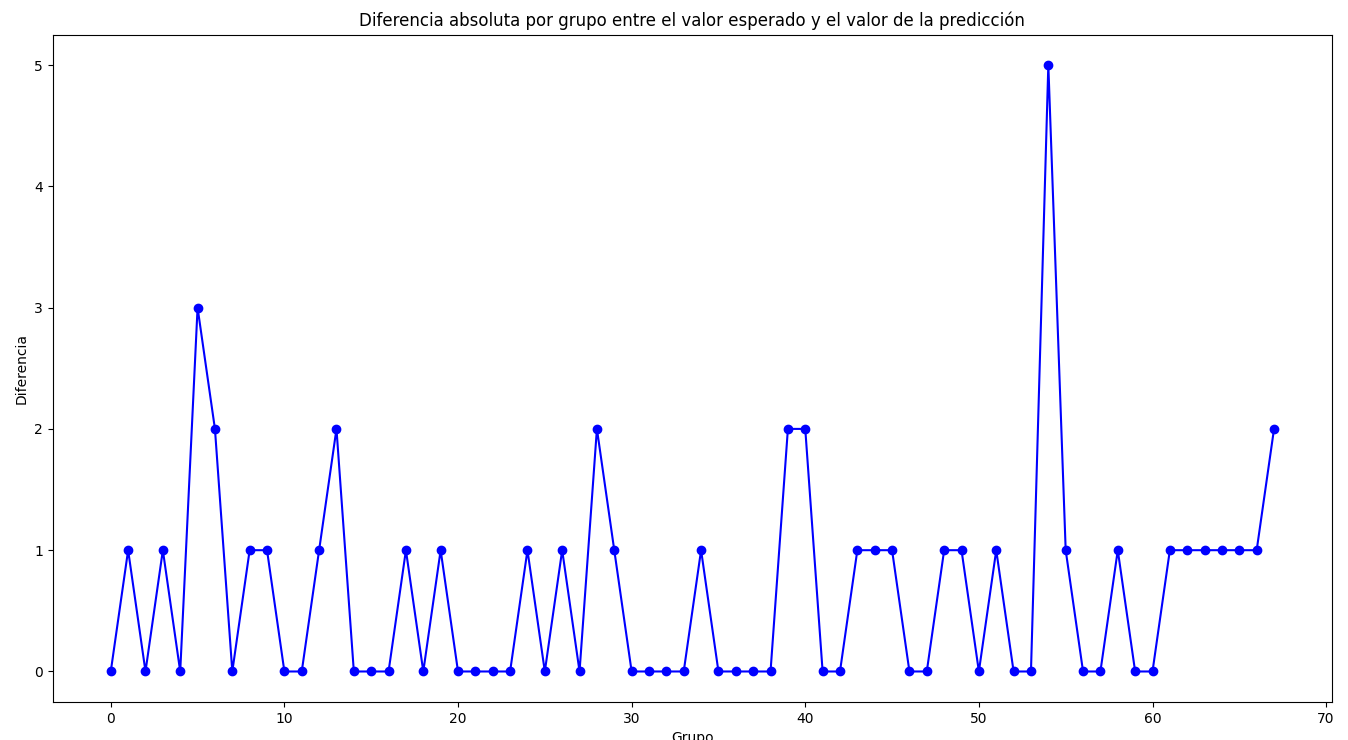
\includegraphics[width=\columnwidth]{assets/absolutas678.png}
    \caption{Gráfico de diferencias absolutas entre las recomendaciones del sistema y las preferencias del usuario. Calificaciones 6, 7, 8.}
    \label{fig:absolutas}
\end{figure}

Lo observado permite concluir que el sistema, en general, ofrece recomendaciones razonablemente precisas en la mayoría de los casos.

\textbf{Tabla de Resultados}

En la Tabla \ref{tab:resultados} se presenta
un resumen cuantitativo de los resultados. Se muestran 
las predicciones, valores reales, diferencias y 
diferencias absolutas para 25 grupos confeccionados y 
las películas seleccionadas. Los resultados completos 
pueden verse en el archivo \textbf{Grupos678.xlsx} en la ruta \textbf{report/assets/} a partir del directorio raíz del repositorio de GitHub.

\begin{figure}[h]
    \centering
    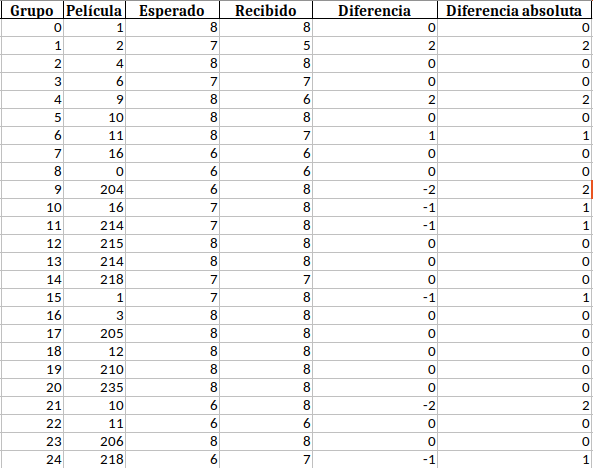
\includegraphics[width=\columnwidth]{assets/tabla678.png}
    \caption{Resumen cuantitativo de los resultados del sistema de recomendación. Calificaciones 6, 7, 8.}
    \label{tab:resultados}
\end{figure}

\textbf{Otras métricas}:
\begin{itemize}
    \item \textbf{MSE (Error Cuadrático Medio): 0.657}: Este valor indica el promedio de los errores al cuadrado entre las predicciones del sistema y los valores reales. El MSE es sensible a errores grandes, ya que estos se amplifican al ser elevados al cuadrado. Un valor de 0.657 implica que, en promedio, las diferencias entre las recomendaciones del sistema y las preferencias reales de los usuarios son moderadamente bajas. Sin embargo, aún existen algunos errores significativos que deben ser corregidos para mejorar la precisión del sistema de recomendación. \cite{tesis_sistema_recomendador_hibrido}
    \item \textbf{MAE (Error Medio Absoluto): 0.486}: Esta métrica refleja el error medio absoluto entre las predicciones y los valores reales, lo cual ofrece una interpretación más intuitiva de la precisión del modelo. En este caso, el valor de 0.486 indica que, en promedio, la desviación entre la predicción y las preferencias reales de los usuarios es de aproximadamente 0.49 unidades. Este valor es más fácil de interpretar que el MSE, y nos muestra que las predicciones del sistema son razonablemente precisas, aunque pueden ser perfeccionadas. \cite{tesis_sistema_recomendador_hibrido}
\end{itemize}

\subsubsection{Resultados con votaciones altas (1, 2, 3)\\}

\textbf{Diferencias}

En la Figura \ref{fig:diferencias2}, se muestran las diferencias entre las recomendaciones sugeridas por el sistema y las expectativas del usuario al analizar las películas con calificaciones bajas (1, 2, 3). 

\begin{figure}[h]
    \centering
    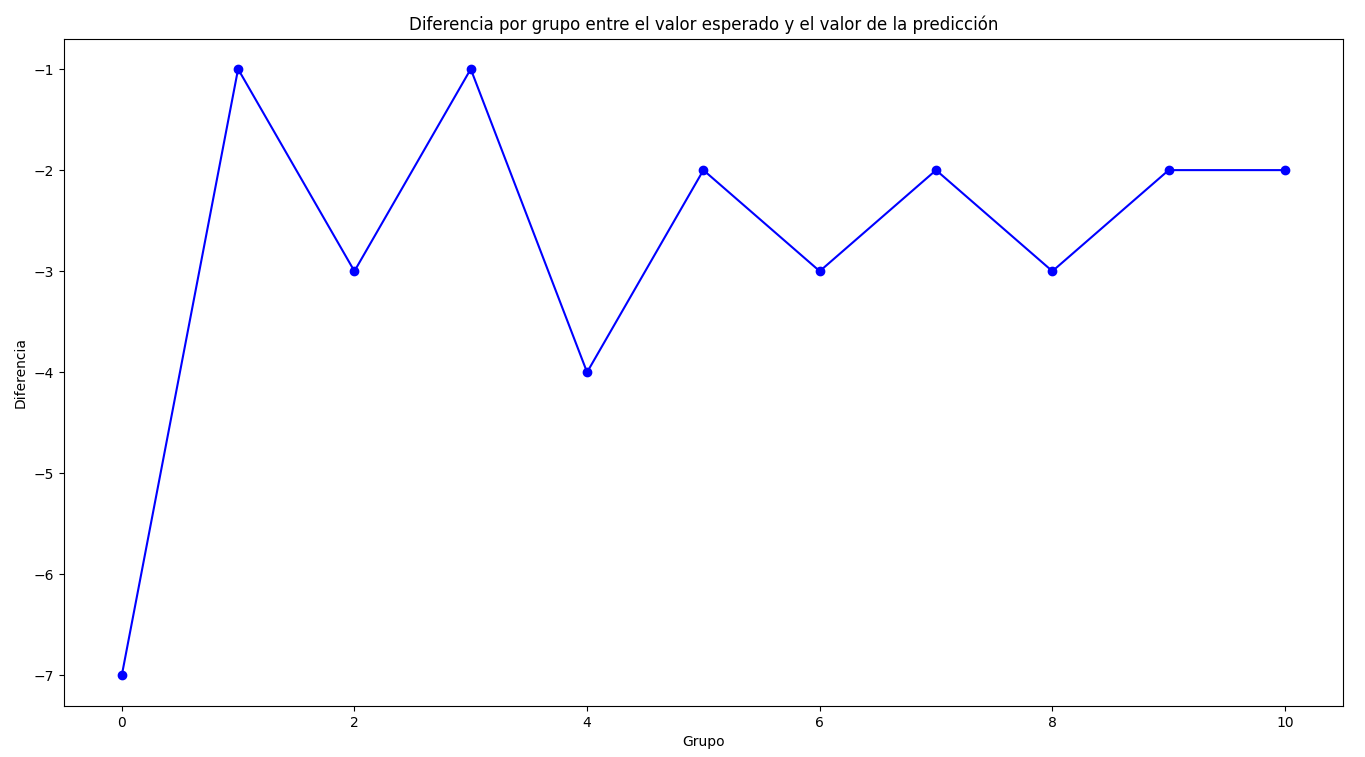
\includegraphics[width=\columnwidth]{assets/Diferencias123.png}
    \caption{Gráfico de diferencias entre las recomendaciones del sistema y las preferencias reales del usuario. Calificaciones 1, 2, 3.}
    \label{fig:diferencias2}
\end{figure}

El análisis indica que el método manifiesta un rendimiendo no tan bueno a la hora de predecir las calificaciones de estas películas, pues en los experimentos siempre predijo valores superiores a los reales. Sin embargo se observa que en algunos casos las diferencias son pequeñas.

\textbf{Diferencias absolutas}

La Figura \ref{fig:absolutas2} muestra las diferencias absolutas, que como en este caso todas las diferencias son negativas, se comporta como mismo la gráfica \ref{fig:diferencias2}

\begin{figure}[h]
    \centering
    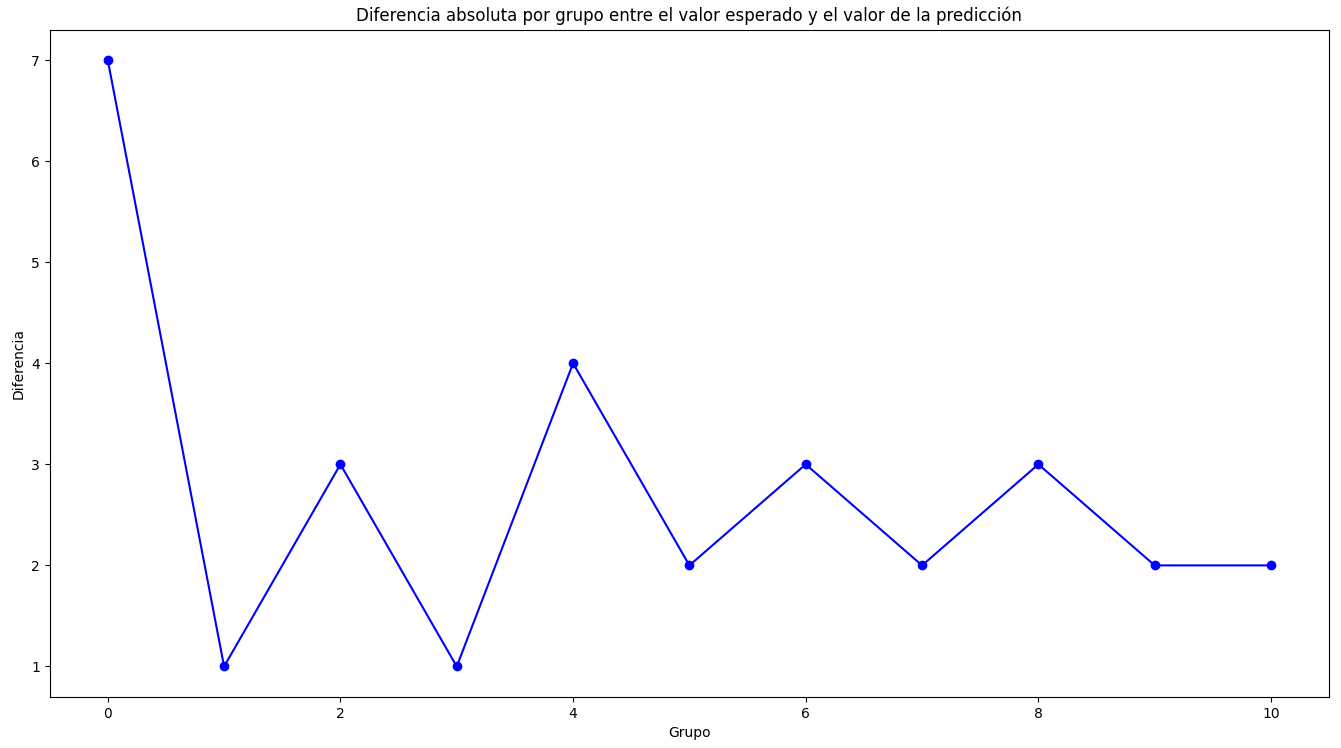
\includegraphics[width=\columnwidth]{assets/absolutas123.png}
    \caption{Gráfico de diferencias absolutas entre las recomendaciones del sistema y las preferencias del usuario. Calificaciones 1, 2, 3.}
    \label{fig:absolutas2}
\end{figure}

\textbf{Tabla de Resultados}

La Tabla \ref{tab:resultados2} muestra el resumen cuantitativo de los resultados para este conjunto de calificaciones. Los resultados completos 
pueden verse en el archivo \textbf{Grupos123.xlsx} en la ruta \textbf{report/assets/} a partir del directorio raíz del repositorio de GitHub.

\begin{figure}[h]
    \centering
    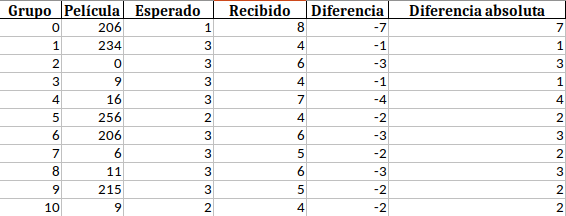
\includegraphics[width=\columnwidth]{assets/tabla123.png}
    \caption{Resumen cuantitativo de los resultados del sistema de recomendación. Calificaciones 1, 2, 3.}
    \label{tab:resultados2}
\end{figure}

\textbf{Otras métricas}:
\begin{itemize}
    \item \textbf{MSE (Error Cuadrático Medio): 9.222}: Este valor elevado del MSE indica que el sistema de recomendación está generando errores significativos al comparar las predicciones con los valores reales. Dado que el MSE eleva al cuadrado las diferencias entre los valores predichos y los valores reales, un valor de 9.222 refleja la presencia de desviaciones grandes en las predicciones. Este resultado es preocupante, ya que significa que, en algunos casos, el sistema está haciendo predicciones muy alejadas de lo que realmente deberían ser.
    \item \textbf{MAE (Error Medio Absoluto): 2.778}: El MAE de 2.778 también es considerablemente alto, lo que sugiere que, en promedio, el sistema se está desviando casi 3 unidades en sus predicciones. Esto implica que las recomendaciones del sistema no están siendo lo suficientemente precisas para ajustarse a las expectativas de los usuarios, lo que puede resultar en una experiencia insatisfactoria para ellos.
\end{itemize}

\subsubsection{Limitaciones}

A pesar de los resultados obtenidos, el sistema de recomendación presenta algunas limitaciones que es importante destacar. Una de las principales dificultades observadas es la capacidad del modelo para realizar predicciones precisas en películas que se espera tengan calificaciones bajas. Este tipo de películas tienden a recibir menos atención de los usuarios, lo que genera un sesgo en los datos disponibles para su análisis y, en consecuencia, afecta la precisión de las predicciones. Esto es especialmente notable cuando se trabaja con conjuntos de datos que no cuentan con suficientes ejemplos de estas películas, dificultando la generalización de las recomendaciones.

Otra limitación importante se refiere a la velocidad de la implementación. Durante la primera ejecución del algoritmo, el procesamiento de los datos y el cálculo de las probabilidades resulta lento debido a la necesidad de precomputar una gran cantidad de información. Sin embargo, una vez que estos cálculos iniciales se han realizado, el sistema es capaz de ejecutar las recomendaciones de manera mucho más eficiente. Esta característica hace que el sistema sea más adecuado para implementarse en computadoras con buenos recursos computacionales, donde la fase de precomputación puede realizarse sin afectar la experiencia del usuario final.

\section{Conclusiones}

El presente trabajo se centró en la hibridación de 
técnicas en sistemas de recomendación, específicamente 
comparando el enfoque probabilístico con la 
factorización matricial en el contexto del filtrado 
colaborativo. Los resultados permiten extraer las 
siguientes conclusiones relevantes:

\begin{itemize}
    \item El enfoque probabilístico, materializado a través del algoritmo \textit{Naive Bayes Collaborative Filtering} (NBCF), no solo demuestra una capacidad comparable en términos de precisión frente a la factorización matricial, sino que también ofrece ventajas adicionales en cuanto a la interpretabilidad de las recomendaciones. Este aspecto resulta fundamental en aplicaciones donde la transparencia es clave para mejorar la experiencia del usuario.
    
    \item La implementación del algoritmo NBCF y su expansión a la recomendación grupal mediante la técnica de \textit{Naive Pooling} (NBP) resuelve de manera eficiente el problema de personalización colectiva. Los resultados experimentales mostraron que este enfoque proporciona recomendaciones coherentes tanto a nivel individual como grupal, lo que es particularmente útil en escenarios de recomendación para familias o grupos de amigos.

    \item En la evaluación sobre el dataset \textit{FilmTrust}, se observó que el enfoque NBCF hibridado mejoró las métricas de rendimiento clave como el error cuadrático medio (MSE) y el error medio absoluto (MAE), especialmente en grupos con votaciones positivas. No obstante, en contextos de votaciones negativas, el rendimiento fue menor, lo que apunta a posibles áreas de mejora en el tratamiento de conjuntos de datos escasos.

    \item A pesar de los buenos resultados en general, el sistema de recomendación presenta limitaciones en la velocidad inicial de procesamiento y en su capacidad para predecir con precisión películas con bajas calificaciones, lo que sugiere la necesidad de optimizaciones adicionales tanto en la fase de precomputación como en la gestión de la dispersión de datos (\textit{sparsity}) del conjunto.

    \item Finalmente, se destaca la flexibilidad del enfoque probabilístico para integrar nuevas variables y su potencial para aplicaciones futuras en diferentes dominios, extendiendo así las capacidades actuales de los sistemas de recomendación colaborativos.

\end{itemize}

La investigación confirma que la hibridación de técnicas de recomendación, en particular el enfoque probabilístico, ofrece una alternativa robusta y explicativa frente a la factorización matricial, mejorando la capacidad de personalización tanto a nivel individual como grupal, con oportunidades claras de optimización en áreas específicas. Se propuso la extensión del método NBCF para realizar recomendaciones a grupos mediando su hibridación con el método NBP.

\renewcommand\refname{Referencias}

\begin{thebibliography}{4}

    \bibitem{nbcf}
    Valdiviezo-Diaz, P., Ortega, F., Cobos, E., \& Lara-Cabrera, R. (2019). A collaborative filtering approach based on Naïve Bayes classifier. IEEE Access, 7, 108581-108592.
    
    \bibitem{estado_arte_sistemas_recomendacion}
    González, O. E., \& Jacques, S. M. (2017). Estado del arte en los sistemas de recomendación. Res. Comput. Sci., 135, 25-40.
    
    \bibitem{hybrid_collaborative_filtering}
    Ortega, F., Rojo, D., Valdiviezo-Diaz, P., \& Raya, L. (2018). Hybrid collaborative filtering based on users rating behavior. IEEE Access, 6, 69582-69591.
    
    \bibitem{tesis_sistema_recomendador_hibrido}
    Valdiviezo, P. M. (2019). Sistema recomendador híbrido basado en modelos probabilísticos (Doctoral dissertation, Universidad Politécnica de Madrid).

    \bibitem{nbp}
    Samsudin, N. A., \& Bradley, A. P. (2014). Extended naïve bayes for group based classification. In Recent Advances on Soft Computing and Data Mining: Proceedings of The First International Conference on Soft Computing and Data Mining (SCDM-2014) Universiti Tun Hussein Onn Malaysia, Johor, MalaysiaJune 16th-18th, 2014 (pp. 497-505). Springer International Publishing.

    \bibitem{filmtrust}
    J. Golbeck, J. Hendler, “FilmTrust: movie recommendations using trust in web-based social networks”, CCNC 2006, 3rd IEEE Consumer Communications and Networking Conference, 2006, DOI: 10.1109/CCNC.2006.1593032 

    \bibitem{TDUEX_2021_Pajuelo_Holguera}
    Pajuelo Holguera, F. (2021). Sistemas de recomendación basados en filtrado colaborativo: aceleración mediante computación reconfigurable y aplicaciones predictivas sensoriales.

    \bibitem{_Cesar_Enrique_Pita_Perez}
    Perez, C. E. P. (2021). Proyecto de Sistema de Recomendación de Filtrado Colaborativo basado en Machine Learning. INF-FCPN-PGI Revista PGI, 48-51.

    
\end{thebibliography}
    


\end{document}
